\section{Results}

\subsection{Retrieval Matrix}

Figure~\ref{fig:retrieval} and Table~\ref{tab:retrieval} report complete-gold retrieval over all eligible claims. Text RRF improves dense Recall@50 from 0.30283 to 0.32242. Cross-encoder reranking raises it further to 0.33381, but lowers MAP from 0.17439 to 0.12822 and remains below the frozen 0.36160 baseline. The text gate therefore fails.

Image filename retrieval is individually weak, but its errors complement SigLIP2. RRF reaches Recall@50 0.31493 versus 0.21829 for SigLIP2 and 0.22273 for filenames. Its $+0.10109$ gain over the frozen 0.21384 baseline passes the image threshold by a narrow margin. The joint retrieval gate still fails. The final packet oracle F1 is 0.46317 and complete-gold claim coverage is only 0.03663.

\begin{figure*}[t]
\centering
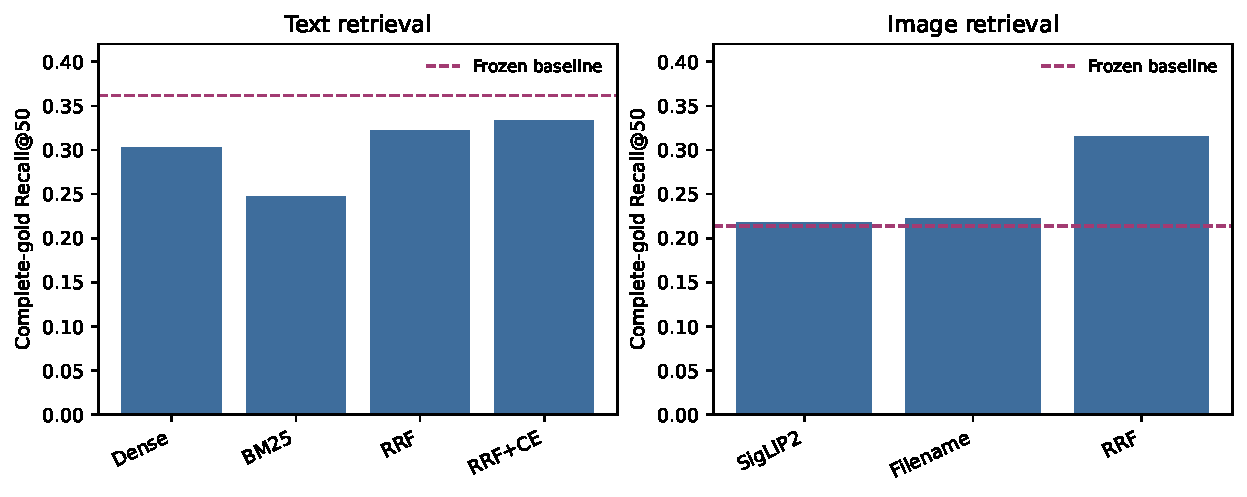
\includegraphics[width=0.92\textwidth]{../research/q1_phase2/figures/retrieval_matrix.pdf}
\caption{Complete-gold Recall@50 for declared text and image retrieval variants. Dashed lines show frozen Phase-1 baselines.}
\label{fig:retrieval}
\end{figure*}

\begin{table}[t]
\centering
\caption{Full retrieval matrix.}
\label{tab:retrieval}
\small
\begin{tabular}{llrr}
\toprule
Modality & Variant & Recall@50 & MAP@100 \\
\midrule
Text & Dense sentence & 0.3028 & 0.1728 \\
Text & BM25 sentence & 0.2478 & 0.1349 \\
Text & Dense--BM25 RRF & 0.3224 & 0.1744 \\
Text & RRF + cross-encoder & 0.3338 & 0.1282 \\
Image & SigLIP2 & 0.2183 & 0.0916 \\
Image & Filename BGE-M3 & 0.2227 & 0.1154 \\
Image & SigLIP2--filename RRF & 0.3149 & 0.1414 \\
\bottomrule
\end{tabular}

\end{table}

\subsection{Scorer and Calibration Gate}

The selected scorer improves model-selection average precision over the shared logistic control in every seed. Seed 13 selects modality-specific logistic scoring; the other four select the cross-encoder-augmented family. Modality temperature scaling improves or preserves Brier score in every seed. Validation Brier decreases from 0.15774--0.16728 raw to 0.15184--0.16295 calibrated. The scorer gate passes, showing that the negative selector result is not caused by retaining the original shared scorer unchanged.

\subsection{Matched Selector Matrix}

Table~\ref{tab:selector} gives five-seed validation means. Fixed top-5 reaches F1 0.16435. Calibrated thresholding is strongest at 0.17863 and improves on fixed by 0.01429, with 95\% CI $[0.01048,0.01814]$. The learned count head over-selects 32.83 items and performs worst.

Original CEFES selects 26.81 items and obtains 0.12227 F1. Size penalties reduce the mean set to 14.89 and improve F1 to 0.14718. \method{} further reduces repeated-source output to 14.73 items but obtains 0.14698 F1. Its mean selected/gold ratio is 1.1809, so the set-size safety condition passes. It nevertheless trails fixed by 0.01737; every seed effect is negative and the aligned CI is $[-0.02264,-0.01222]$.

\begin{table}[t]
\centering
\caption{Five-seed mean complete-gold selector results.}
\label{tab:selector}
\small
\resizebox{\columnwidth}{!}{\begin{tabular}{lrrrr}
\toprule
Method & Precision & Recall & F1 & Selected \\
\midrule
Fixed top-5 & 0.2460 & 0.1718 & 0.1643 & 5.00 \\
Calibrated threshold & 0.2816 & 0.1794 & 0.1786 & 5.53 \\
Learned count & 0.0907 & 0.2818 & 0.1087 & 32.83 \\
CEFES & 0.1002 & 0.2792 & 0.1223 & 26.81 \\
Size-penalized CEFES & 0.1435 & 0.2433 & 0.1472 & 14.89 \\
RC-CEFES & 0.1438 & 0.2421 & 0.1470 & 14.73 \\
\bottomrule
\end{tabular}
}
\end{table}

\begin{figure}[t]
\centering
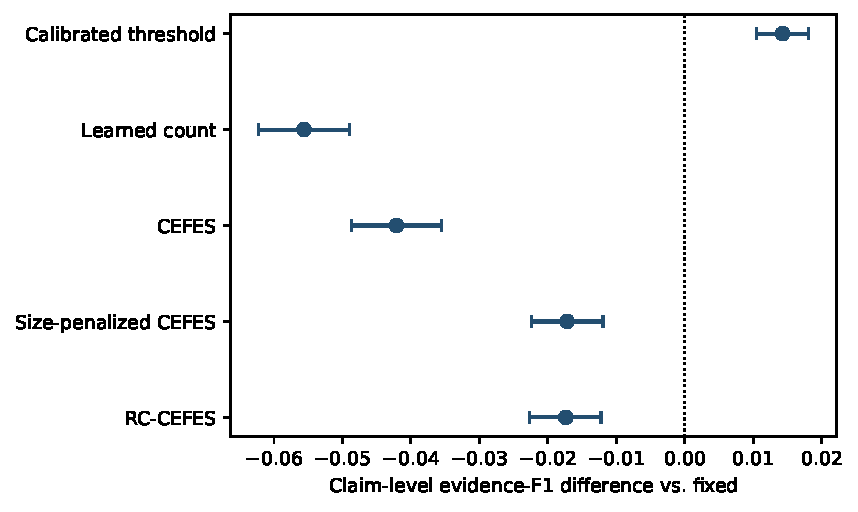
\includegraphics[width=\columnwidth]{../research/q1_phase2/figures/selector_effects.pdf}
\caption{Seed-aligned evidence-F1 effects against fixed top-5. All Holm-adjusted $p$ values are 0.0010.}
\label{fig:selector-effects}
\end{figure}

\begin{table}[t]
\centering
\caption{Seed-aligned selector effects against fixed.}
\label{tab:selector-effects}
\small
\resizebox{\columnwidth}{!}{\begin{tabular}{lrrrr}
\toprule
Method vs. fixed & Mean & 95\% lower & 95\% upper & Holm $p$ \\
\midrule
Calibrated threshold & +0.0143 & +0.0105 & +0.0181 & 0.0010 \\
Learned count & -0.0556 & -0.0623 & -0.0490 & 0.0010 \\
CEFES & -0.0421 & -0.0486 & -0.0355 & 0.0010 \\
Size-penalized CEFES & -0.0172 & -0.0224 & -0.0119 & 0.0010 \\
RC-CEFES & -0.0174 & -0.0226 & -0.0122 & 0.0010 \\
\bottomrule
\end{tabular}
}
\end{table}

\subsection{Shared-Verifier Safeguard}

The mean \method{}--fixed verifier change is $+0.00435$ macro-F1. The aligned interval, $[-0.01126,0.02005]$, crosses zero and its lower bound is below the $-0.01$ margin. The non-inferiority safeguard therefore fails, even though the point estimate is positive. Calibrated thresholding has the highest verifier macro-F1 in every seed.

\begin{figure}[t]
\centering
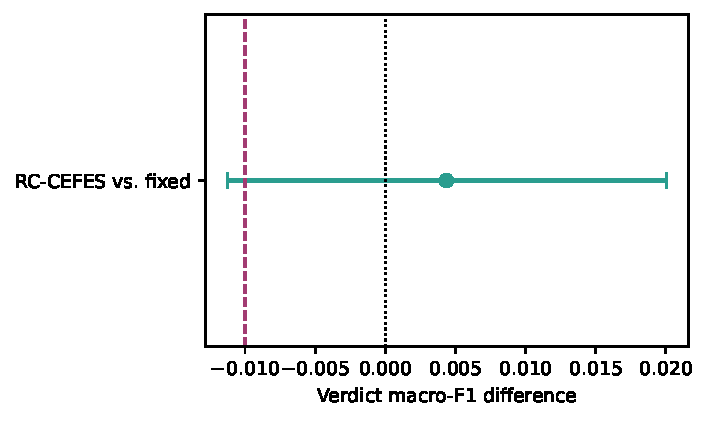
\includegraphics[width=\columnwidth]{../research/q1_phase2/figures/verifier_noninferiority.pdf}
\caption{Shared-verifier effect. The dashed line is the $-0.01$ non-inferiority margin.}
\label{fig:verifier}
\end{figure}

\subsection{Controlled Robustness Diagnostics}

The post-outcome diagnostic protocol perturbs frozen packets without refitting. Figure~\ref{fig:robustness} shows that \method{} remains below fixed for width 20/40, text-only or image-only packets, removal of retrievable gold, and both rank-preserving temperature shifts. At width 10 its interval reaches zero. Duplicating the top three items also yields an interval containing zero, consistent with the redundancy penalty becoming useful.

Promoting five known non-gold candidates to the highest scores produces a large \method{} advantage ($+0.13736$). This is not evidence of ordinary superiority: the intervention deliberately fills fixed top-5 with distractors, while the larger adaptive set can still recover evidence below them. It locates a boundary where a variable set is robust to catastrophic early ranking error.

\begin{figure*}[t]
\centering
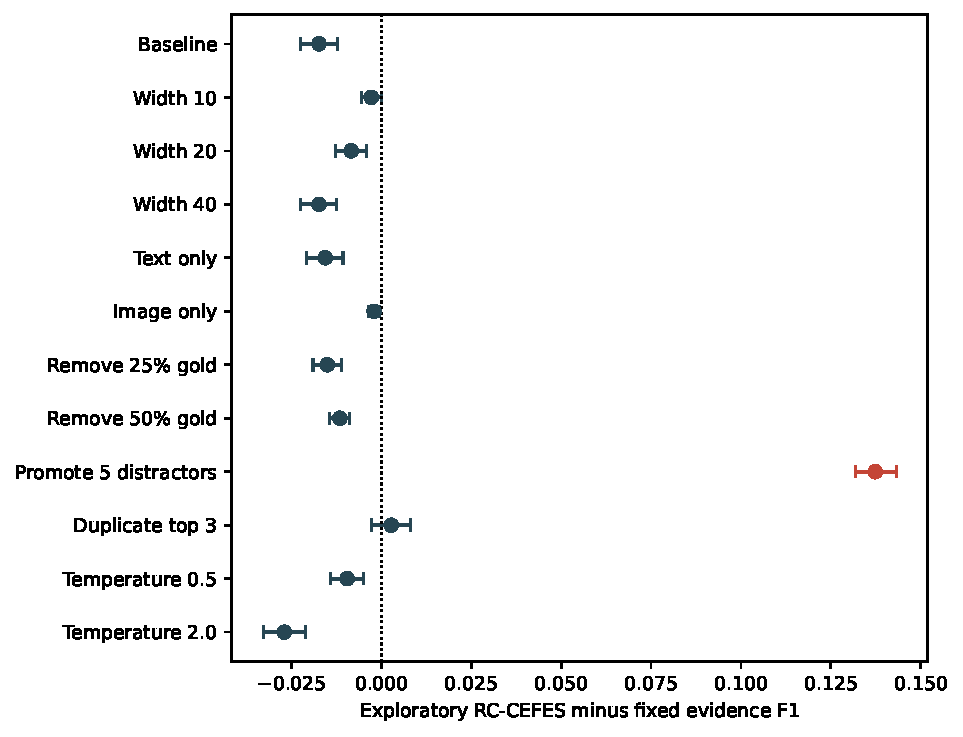
\includegraphics[width=0.82\textwidth]{../research/q1_phase2/figures/robustness_effects.pdf}
\caption{Exploratory five-seed effects under frozen packet perturbations. The highlighted condition deliberately promotes known distractors and has no confirmatory status.}
\label{fig:robustness}
\end{figure*}

\subsection{Reproduction, External Gate, and Final Decision}

A clean run rebuilds retrieval rankings, candidate features, five-seed scorer/selector records, verifier checkpoints, and predictions in a separate namespace. Twenty-seven core artifacts match byte-for-byte. The two label-blind prejoin manifests match after normalizing their expected output-path strings. All six independent audits pass.

AVerImaTeC and MMCV pass licensing/relevance screening but not unchanged-protocol compatibility. AVerImaTeC has no usable released blind test and represents evidence as QA-supported web sources. MMCV adds table evidence, lacks an official fitting/test split, and reports an open-book condition with gold evidence. No external outcome is claimed.

Table~\ref{tab:gate} gives the final conjunctive decision. Text retrieval, selector superiority, and verifier non-inferiority fail. The formal test remains sealed.

\begin{table}[t]
\centering
\caption{Final development gate. Every condition is required.}
\label{tab:gate}
\small
\begin{tabular}{p{0.76\columnwidth}c}
\toprule
Condition & Status \\
\midrule
Text Recall@50 gain at least +0.10 & \textbf{Fail} \\
Image Recall@50 gain at least +0.10 & Pass \\
Selected scorer improves MAP in every seed & Pass \\
Calibrated Brier score is non-worse in every seed & Pass \\
Mean RC-CEFES evidence-F1 gain at least +0.015 & \textbf{Fail} \\
RC-CEFES evidence effect positive in every seed & \textbf{Fail} \\
Seed-aligned evidence interval lower bound above zero & \textbf{Fail} \\
Mean selected/gold evidence ratio no more than 2 & Pass \\
Verifier interval lower bound above -0.01 & \textbf{Fail} \\
Clean end-to-end reproduction & Pass \\
\bottomrule
\end{tabular}

\end{table}
